\documentclass[11pt,a4paper]{article}
\usepackage[utf8]{inputenc}
\usepackage[T1]{fontenc}
\usepackage[spanish]{babel}
\usepackage[margin=2.2cm]{geometry}
\usepackage{xcolor}
\usepackage{tcolorbox}
\usepackage{amsmath}
\usepackage{booktabs}
\usepackage{array}
\usepackage{graphicx}
\usepackage{listings}
\usepackage{hyperref}
\usepackage{fancyhdr}
\usepackage{float}

\definecolor{azul}{HTML}{0F2A4A}
\definecolor{celeste}{HTML}{1F6FA8}
\definecolor{naranja}{HTML}{D98A12}
\definecolor{fondoc}{HTML}{F4F6F9}

\lstset{
  language=Verilog,
  basicstyle=\ttfamily\footnotesize,
  keywordstyle=\color{celeste}\bfseries,
  commentstyle=\color{gray}\itshape,
  numbers=left, numberstyle=\tiny\color{gray},
  breaklines=true, frame=single, backgroundcolor=\color{fondoc},
  tabsize=2, showstringspaces=false
}

\pagestyle{fancy}
\fancyhf{}
\renewcommand{\headrulewidth}{0.4pt}
\fancyhead[L]{\small Pr\'actica 3. Sistemas Embebidos}
\fancyhead[R]{\small UDLAP}
\fancyfoot[C]{\thepage}

\newcommand{\tbox}[2]{%
  \begin{tcolorbox}[colback=fondoc,colframe=#1,title=#2,fonttitle=\bfseries,boxrule=0.6pt,arc=2pt]
}

\begin{document}

% ---------------- PORTADA ----------------
\begin{center}
  \colorbox{azul}{\parbox{0.92\textwidth}{\centering\color{white}\bfseries\large\strut UNIVERSIDAD DE LAS AM\'ERICAS PUEBLA\strut}}\\[1.2em]
  {\LARGE\bfseries\color{celeste} PR\'ACTICA 3}\\[0.3em]
  {\small Sistemas embebidos con FPGA}\\[1.2em]
  \fcolorbox{celeste}{fondoc}{\parbox{0.9\textwidth}{\centering\color{celeste}\large\bfseries\strut Contador ascendente--descendente de 9 bits con signo\\[0.2em]
  Intervalo de $-256$ a $255$ en la DE10-Lite\strut}}
\end{center}

\vspace{1.2em}

\begin{tabular}{@{}p{3.2cm}p{11.8cm}@{}}
  \textbf{Integrantes:} & Roberto Orozco Ram\'irez \quad ID: 184595\\
                        & Adam Del Pozo Ontiveros \quad ID: 185611\\
                        & Enrique Bernal Mart\'in Prieto \quad ID: 184878\\[0.4em]
  \textbf{Carrera:}     & Ingenier\'ia en Sistemas Computacionales\\
  \textbf{Materia:}     & Sistemas Embebidos\\
  \textbf{Fecha:}       & 16 de octubre de 2026\\
\end{tabular}

\vspace{0.8em}
\tbox{celeste}{Resumen}
En esta pr\'actica se dise\~n\'o, simul\'o e implement\'o un contador ascendente--descendente de 9 bits con signo en Verilog. El valor recorre el intervalo completo de complemento a dos, de $-256$ a $255$, con control de reinicio, pausa, conteo ascendente y descendente, y un selector de actualizaci\'on de 1 s o 100 ms. El valor se muestra en decimal en HEX2--HEX0, y HEX3 indica el signo. El dise\~no usa un \'unico reloj de 50 MHz y pulsos de habilitaci\'on (\texttt{tick}) de un ciclo.
\end{tcolorbox}

% ---------------- 1. OBJETIVO ----------------
\section{Objetivo}
Dise\~nar e implementar en Verilog un contador ascendente--descendente de 9 bits con signo, verificar su comportamiento mediante simulaci\'on funcional y demostrarlo en la tarjeta DE10-Lite, incluyendo los l\'imites del intervalo y el cambio de signo.

% ---------------- 2. TEORIA ----------------
\section{Fundamento te\'orico}
\subsection{Representaci\'on con signo en 9 bits}
Un n\'umero de 9 bits en complemento a dos representa $x$ con $-2^{8}\le x\le 2^{8}-1$, es decir, de $-256$ a $255$. El bit m\'as significativo \texttt{count[8]} funciona como bit de signo: vale 0 para no negativos y 1 para negativos. Como hay $2^9=512$ patrones, el rango es sim\'etrico salvo por un patr\'on extra en el lado negativo: $-256 = 1\_0000\_0000$, que no tiene contraparte positiva.

Como la aritm\'etica es modular, el contador da la vuelta sin saturar:
\[
255 + 1 \longrightarrow -256, \qquad -256 - 1 \longrightarrow 255.
\]

\subsection{Unidad de control y ruta de datos}
La unidad de control es una m\'aquina de estados con tres estados: \textbf{PAUSA} (conserva el valor), \textbf{ASCENDENTE} (suma 1 en cada \texttt{tick}) y \textbf{DESCENDENTE} (resta 1 en cada \texttt{tick}). La ruta de datos es un registro con signo de 9 bits que solo cambia cuando llega un \texttt{tick}.

\subsection{Pulso de habilitaci\'on}
La DE10-Lite entrega un reloj de 50 MHz. Para un intervalo $T$ el n\'umero de ciclos es $N=f_{\text{CLK}}\,T$:
\[
N_{1\,\text{s}} = 50\,000\,000, \qquad N_{100\,\text{ms}} = 5\,000\,000.
\]
El divisor cuenta de $0$ a $N-1$ y genera un pulso de un solo ciclo. No se crea ning\'un reloj nuevo, as\'i que todo el dise\~no sigue en el dominio del reloj principal.

\subsection{Acondicionamiento de botones}
Los pulsadores mec\'anicos rebotan y son as\'incronos respecto al reloj. El dise\~no usa un sincronizador de dos flip-flops, un filtro antirrebote de 10 ms (500\,000 ciclos) y un pulso de un ciclo por pulsaci\'on v\'alida.

% ---------------- 3. MATERIAL ----------------
\section{Material y software}
\begin{itemize}
  \item Intel Quartus Prime (proyecto para el dispositivo 10M50DAF484C7G de la DE10-Lite).
  \item Tarjeta FPGA DE10-Lite, cable USB Blaster y manual de la tarjeta.
  \item Icarus Verilog 12.0 para simulaci\'on funcional.
\end{itemize}

% ---------------- 4. DISE\~NO ----------------
\section{Dise\~no implementado}
\subsection{Arquitectura y m\'aquina de estados}
\begin{itemize}
  \item \textbf{\texttt{tick\_generator}}: genera \texttt{tick} de un ciclo cada 1 s o cada 100 ms seg\'un \texttt{speed\_sel}. Se usa \texttt{>=} en la comparaci\'on para que un cambio del selector no deje al divisor esperando un valor ya rebasado. En pausa el divisor se mantiene en cero.
  \item \textbf{\texttt{signed\_counter\_fsm}}: FSM de tres estados y contador con signo. La prioridad es RESET $>$ PAUSA $>$ INCREMENTO $>$ DECREMENTO. El contador solo se actualiza en \texttt{tick}.
  \item \textbf{\texttt{signed\_display\_9bit}}: convierte el valor a magnitud decimal (centenas, decenas y unidades) y a 7 segmentos activos en bajo. HEX3 enciende solo el segmento \emph{g} cuando el n\'umero es negativo. Los ceros a la izquierda se apagan.
  \item \textbf{\texttt{button\_onepulse}}: sincronizador de dos FF, antirrebote de 10 ms y pulso de un ciclo.
  \item \textbf{\texttt{counter\_9bit\_top}}: m\'odulo superior que integra todos los bloques.
\end{itemize}

Asignaci\'on de recursos usada en la tarjeta: KEY0 = reset, KEY1 = pausa, pulsador GPIO = incremento, pulsador GPIO = decremento, SW0 = selector de frecuencia (0: 1 s, 1: 100 ms). Los n\'umeros de pin se toman del archivo de asignaciones de la DE10-Lite del laboratorio.

\subsection{Tabla de LEDs}
\begin{center}
\begin{tabular}{@{}llp{7.5cm}@{}}
\toprule
LED & Se\~nal & Significado\\
\midrule
LEDR[0] & PAUSA & Estado de pausa\\
LEDR[1] & ASCENDENTE & Conteo hacia arriba\\
LEDR[2] & DESCENDENTE & Conteo hacia abajo\\
LEDR[3] & \texttt{speed\_sync} & Actualizaci\'on cada 100 ms\\
LEDR[9] & \texttt{count[8]} & N\'umero negativo\\
\bottomrule
\end{tabular}
\end{center}

% ---------------- 5. SIMULACION ----------------
\section{Simulaci\'on funcional}
Se simularon dos testbenches con Icarus Verilog. El primero (\texttt{tb\_counter\_fsm.v}) sigue la tabla de pruebas de la pr\'actica. El segundo (\texttt{tb\_display\_tick.v}) verifica el decodificador de 7 segmentos y el periodo del tick. Ambos reportan \texttt{PASS}/\texttt{FAIL} autom\'aticamente.

\subsection{Resultados de la tabla de pruebas}
\begin{center}
\begin{tabular}{@{}llrl@{}}
\toprule
Valor actual & Evento & Valor obtenido & Estado\\
\midrule
0 & RESET & 0 & PAUSA\\
0 & INC y despu\'es tick & 1 & ASCENDENTE\\
58 & tick & 59 & ASCENDENTE\\
255 & tick & $-256$ & ASCENDENTE\\
0 & DEC y despu\'es tick & $-1$ & DESCENDENTE\\
$-58$ & tick & $-59$ & DESCENDENTE\\
$-256$ & tick & 255 & DESCENDENTE\\
45 & PAUSA y varios ticks & 45 & PAUSA\\
$-123$ & RESET & 0 & PAUSA\\
\bottomrule
\end{tabular}
\end{center}

La salida completa de la simulaci\'on del FSM dice: \emph{TODAS LAS PRUEBAS PASARON} (16 de 16 verificaciones). Adem\'as se prob\'o que PAUSA tiene prioridad sobre INCREMENTO cuando llegan en el mismo ciclo.

\subsection{Decodificador y periodo del tick}
\begin{center}
\begin{tabular}{@{}rllll@{}}
\toprule
Valor & HEX3 & HEX2 & HEX1 & HEX0\\
\midrule
255 & (apagado) & 2 & 5 & 5\\
$-256$ & \textbf{-} & 2 & 5 & 6\\
$-1$ & \textbf{-} & (apagado) & (apagado) & 1\\
0 & (apagado) & (apagado) & (apagado) & 0\\
45 & (apagado) & (apagado) & 4 & 5\\
$-123$ & \textbf{-} & 1 & 2 & 3\\
100 & (apagado) & 1 & 0 & 0\\
\bottomrule
\end{tabular}
\end{center}

El periodo medido entre dos ticks a 100 ms fue de \textbf{5\,000\,000 ciclos}, igual al valor esperado.

% ---------------- 6. DEMOSTRACION ----------------
\section{Demostraci\'on en la DE10-Lite}
\subsection{Evidencia en la tarjeta}
\begin{figure}[H]
  \centering
  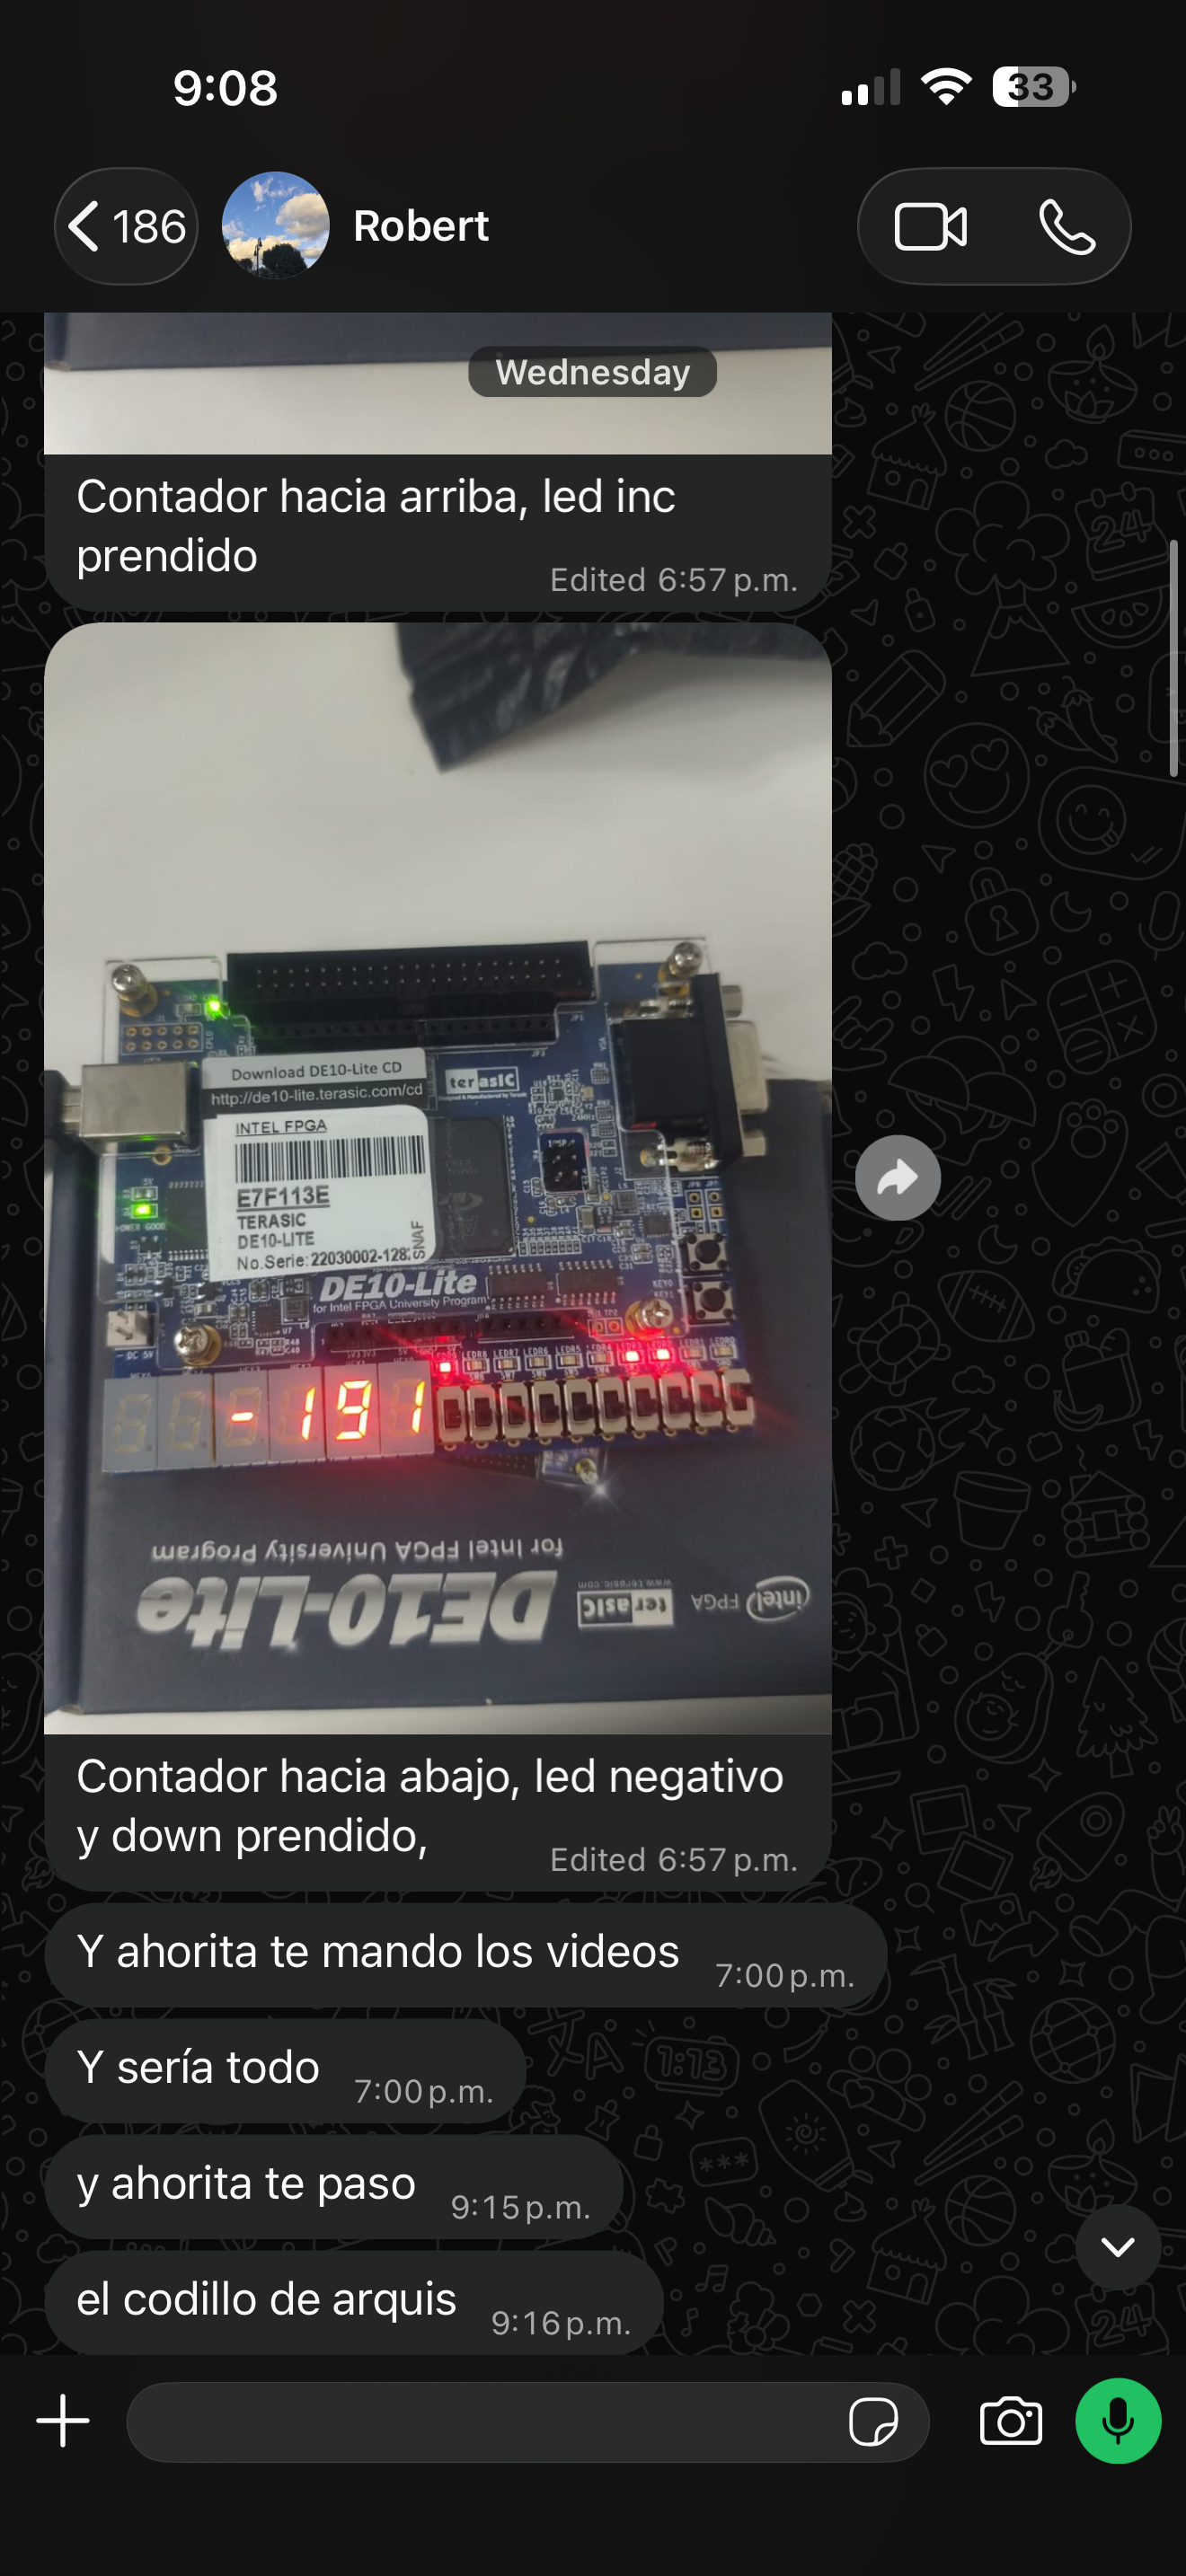
\includegraphics[width=0.55\textwidth]{fotos/contador_abajo.png}
  \caption{Conteo descendente con valor negativo ($-191$). HEX3 muestra el signo, LEDR[9] est\'a encendido y LEDR[2] (DESCENDENTE) tambi\'en.}
\end{figure}
\begin{figure}[H]
  \centering
  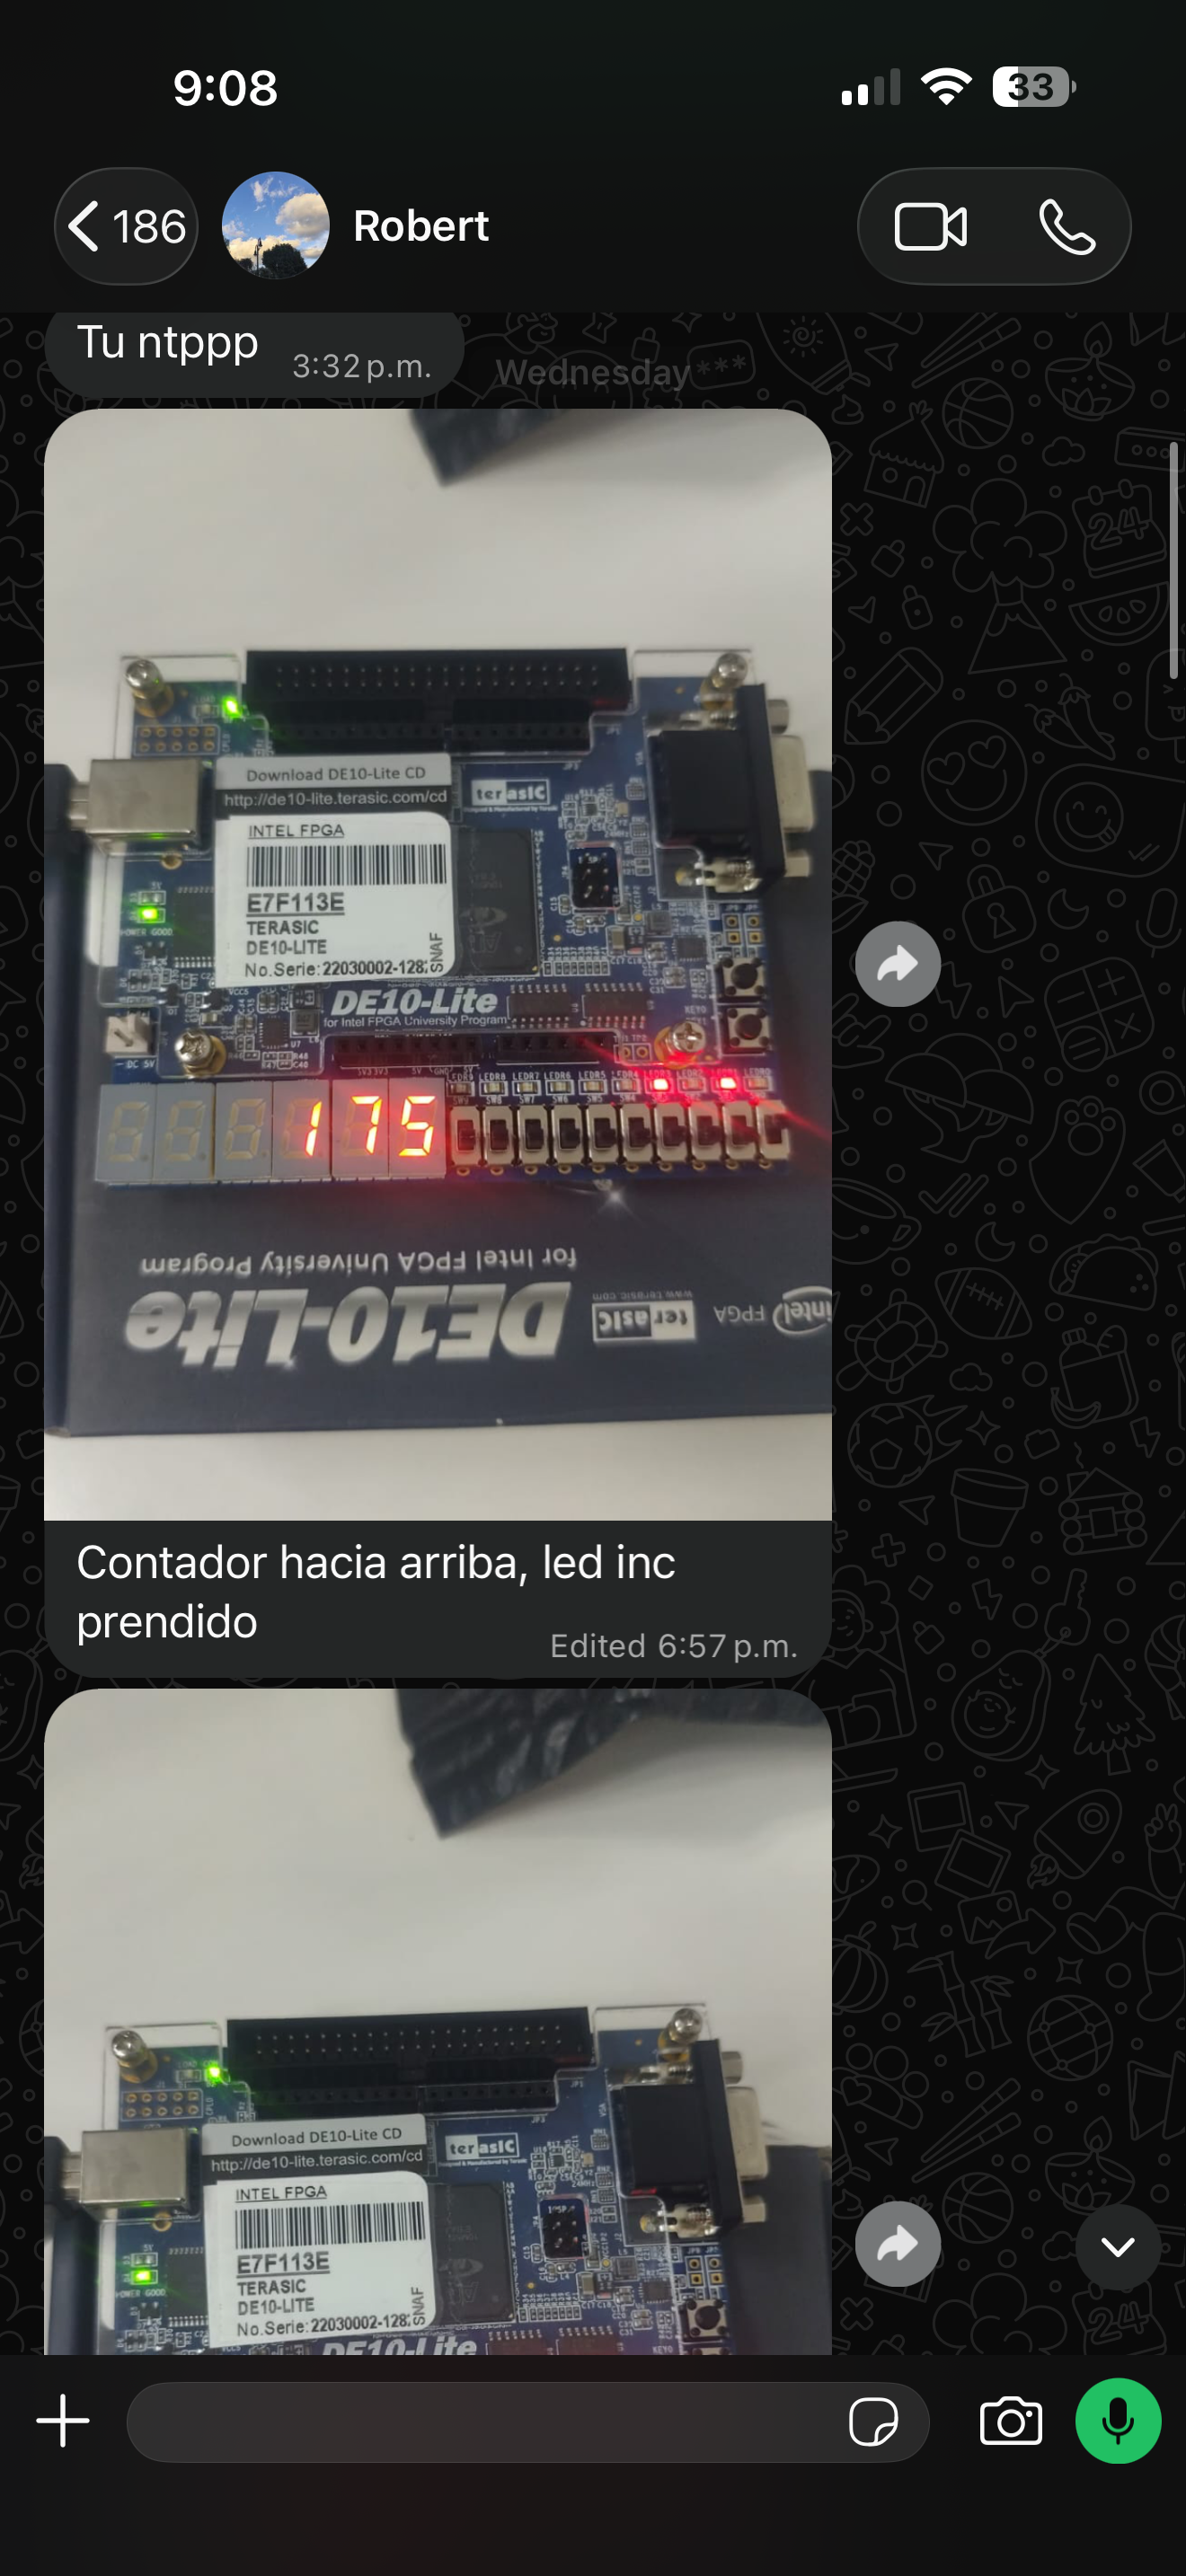
\includegraphics[width=0.55\textwidth]{fotos/contador_arriba.png}
  \caption{Conteo ascendente con valor positivo ($175$). LEDR[1] (ASCENDENTE) est\'a encendido.}
\end{figure}

\subsection{Pruebas en hardware}
\begin{itemize}
  \item Conteo descendente con valor negativo: el display muestra $-191$, con el signo en HEX3 y el LED de signo, DESCENDENTE y el LED de negativo encendidos.
  \item Conteo ascendente con valor positivo: el display muestra $175$ y LEDR[1] (ASCENDENTE) est\'a encendido.
\end{itemize}

% ---------------- 7. CONCLUSIONES
\section{Conclusiones}
La representaci\'on en complemento a dos explica el rango asim\'etrico de $-256$ a $255$ y el comportamiento modular al cruzar los l\'imites. Separar la unidad de control de la ruta de datos facilit\'o verificar la FSM por separado, y el uso de un pulso \texttt{tick} mantuvo un \'unico dominio de reloj de 50 MHz, sin relojes derivados por l\'ogica combinacional.

% ---------------- 8. CUESTIONARIO ----------------
\section{Cuestionario}
\begin{enumerate}
  \item \textbf{¿Por qu\'e 9 bits con signo representan de $-256$ a $255$ y no de $-255$ a $255$?} Con 9 bits hay $2^9=512$ patrones. Se reparten $256$ negativos ($-256$ a $-1$), $0$ y $255$ positivos. El patr\'on $1\_0000\_0000$ representa $-256$, que no tiene contraparte positiva, as\'i que el rango no es sim\'etrico.
  \item \textbf{¿Qu\'e patr\'on binario representa $-256$?} $1\_0000\_0000$ (bit de signo en 1 y el resto en 0).
  \item \textbf{¿Qu\'e ocurre al incrementar 255 y al decrementar $-256$?} La aritm\'etica es modular: $255+1$ da $-256$ y $-256-1$ da $255$. No hay saturaci\'on; el registro simplemente da la vuelta.
  \item \textbf{¿Qu\'e diferencia hay entre generar un reloj nuevo y generar un pulso de habilitaci\'on?} Un reloj derivado de l\'ogica combinacional tiene retrasos distintos a los del reloj principal, lo que causa sesgo de reloj y violaciones de temporizaci\'on, y crea dominios de reloj que hay que sincronizar. Un pulso de habilitaci\'on de un ciclo mantiene todo el dise\~no en el dominio de 50 MHz: los registros siguen cambiando en el mismo flanco y solo se actualizan cuando el pulso est\'a activo.
  \item \textbf{¿Por qu\'e deben sincronizarse las entradas de los botones?} Son as\'incronas respecto al reloj de la FPGA. Si cambian justo cerca de un flanco, el flip-flop puede entrar en metaestabilidad. Un sincronizador de dos flip-flops reduce ese riesgo.
  \item \textbf{¿Qu\'e problema evita el circuito antirrebote?} Un pulsador mec\'anico produce varios cambios r\'apidos en una sola pulsaci\'on. Sin filtro, el contador contar\'ia varias pulsaciones donde solo hubo una. El filtro de 10 ms acepta el cambio solo cuando la se\~nal permanece estable.
  \item \textbf{¿Cu\'antos ciclos de 50 MHz corresponden a 100 ms?} $0.1\,\text{s}\times 50\times 10^{6}\,\text{Hz} = 5\,000\,000$ ciclos.
  \item \textbf{¿Qu\'e recursos adicionales pueden requerir los operadores de divisi\'on y m\'odulo durante la s\'intesis?} Como el divisor y el m\'odulo son por constantes, se sintetizan como l\'ogica de multiplicaci\'on por constantes y sumadores, lo que consume elementos l\'ogicos adicionales. En el decodificador de displays, este costo es peque\~no; un algoritmo \emph{double dabble} puede reducirlo si el \'area es cr\'itica.
\end{enumerate}

% ---------------- 9. BIBLIOGRAFIA ----------------
\section{Bibliograf\'ia}
\begin{itemize}
  \item M. M. Mano y M. D. Ciletti, \emph{Digital Design: With an Introduction to the Verilog HDL, VHDL, and SystemVerilog}, 6.a ed., Pearson, 2018.
  \item S. Brown y Z. Vranesic, \emph{Fundamentals of Digital Logic with Verilog Design}, 3.a ed., McGraw-Hill, 2014.
  \item Terasic, \emph{DE10-Lite User Manual}.
  \item Intel, \emph{Quartus Prime Design Software Documentation}.
\end{itemize}

% ---------------- ANEXO ----------------
\newpage
\appendix
\section{C\'odigo fuente}
\subsection{M\'odulo superior}
\lstinputlisting{../rtl/counter_9bit_top.v}
\subsection{Unidad de control y ruta de datos}
\lstinputlisting{../rtl/signed_counter_fsm.v}
\subsection{Decodificador de displays}
\lstinputlisting{../rtl/signed_display_9bit.v}
\subsection{Generador de tick}
\lstinputlisting{../rtl/tick_generator.v}
\subsection{Antirrebote}
\lstinputlisting{../rtl/button_onepulse.v}

\end{document}
